\documentclass[a4paper, 13pt]{article}
\usepackage[a4paper,top=50pt,bottom=50pt,left=30pt,right=30pt]{geometry}

\usepackage[french]{babel}

\usepackage{mathptmx}
\usepackage{enumitem}
\usepackage{graphicx}

\newcommand{\q}[1]{``#1''}
\begin{document}
\title{Compte rendu de la séance 2}
\author{Ecaterina GUPCA, Alice MERAUD, Jean COSTREL DE CORAINVILLE, Romain REN et Faustin MILLET}
\maketitle

\section{Compte rendu vidéo 1}
Dans cette vidéo, la femme nous explique comment le livre va de l’écrivain à nos mains. Le chemin est le suivant, d'abord l'écrivain puis l'éditeur et enfin le libraire.

Quand l'auteur a fini son manuscrit, il le confie à un éditeur qui le met en forme, l'imprime et le fait connaître. Il peut faire appel à un distributeur, ou diffuseur avec qui il signe un contrat précisant l'exclusivité, la durée, le prix du transport ou encore la remise.

Pour les livres publiées à l'étranger le prix est décidé par l’éditeur lui-même. L'industrie du livre met en marché plus de 30 0000 nouveautés différentes. 

La diffusion s'occupe de plusieurs tâches :
\begin{enumerate}
    \item Prospection de clientèles
    \item Détermination des remises accordées aux clients
    \item Représentation de la production des éditeurs
    \item Promotions des ventes/sollicitation des médias
    \item Publicité
    \item Commande et établissement du prix de vente suggérer pour les livres importé
\end{enumerate}

La distribution s'occupe d'autres tâches comme :
\begin{enumerate}
    \item L'ensemble des activités logistiques exercées pour acheminer des livres sur les lieux de vente
    \item Réception et entreposage des livres
    \item Exécution des commandes
    \item Livraison des marchandises
    \item Facturation et recouvrement des comptes clients
\end{enumerate}

L'Association des Distributeurs Exclusive de Livre en Langue Française ou ADELF représente 23 entreprises membres dont 17 qui sont diffuseurs et distributeurs, 5 qui sont juste diffuseurs et une qui est juste distributeur.

\section{Compte rendu vidéo 2}
Secteur de la diffusion/distribution régit par 2 lois fondamentales :
\subsection{Loi sur le droit d’auteur et règlement sur l’importation de livres}
\begin{itemize}
    \item La loi définit les utilisations protégées, les droits exclusifs de distribution de livres font partie des utilisations protégées grâce aux règlements sur l’importation de livres.
    \item Ce règlement protège les titulaires de droits exclusives de distribution sur le marché canadien contre toute forme d’importation parallèle, en contrepartie les distributeurs exclusives doivent traiter dans un temps déterminé les commandes des détaillants.
\end{itemize}
\subsection{Loi sur le développement des entreprises dans le domaine du livre}
\begin{itemize}
    \item Les objectifs de cette loi sont multiples : augmenter l’accessibilité du livre, implanter un réseau de libraires agréées dans tous le Québec, avoir une stabilité ou augmentation du prix du livre et développer une infrastructure dans le domaine du livre. 
    \item De par cette loi, les distributeurs/diffuseurs doivent accorder une remise de 30-40\% aux libraires agréés. 
    \item Les librairies agréées seront les seuls à pouvoir vendre aux acheteurs institutionnels(administrations publiques et établissements publics).
    \item Pour être agréé, il faut remplir certaines conditions, il y a actuellement 215 libraires agréés au Québec.
    \item Fixation d’un système de prix pour limiter les prix de ventes maximaux des livres importés.
\end{itemize}
\section{Questions pour un libraire}
\subsection{Librairie du beau papier Orsay}
\subsubsection{Questions}
\begin{enumerate}
    \item Quand il vous manque un livre demandé par le client comment vous vous le procurez ?
    \item Comment vous vous fournissez en livre ? Est-ce que c'est les éditeurs qui vous les font parvenir, ou bien est-ce que vous devez vous assurez vous-même du cheminement ?
    \item Comment déterminez-vous les livres que vous mettez en avant ? Est-ce que vous choisissez des maisons d'éditions en particulier ?
    \item Comment gérez-vous vos stocks ? Est-ce que chaque maison d'édition utilise les mêmes moyens ?
    \item Quels avantages recherchez-vous quand vous travaillez avec une maison d'édition ?
    \item Comment les tendances du marché par exemple, les tendances de la vente en ligne, ont-elles affecté votre activité de libraire ces dernières années ?
    \item Est que vous préférez travailler avec une maison d'édition directement ?
\end{enumerate}
\subsubsection{Réponses}
\begin{enumerate}
    \item Quand un client vient commander un livre on essaye de le fournir en minimum trois jours, mais ça dépend de la quantité, par exemple si le livre est demandé par un élève de l'école à proximité, on en commande plusieurs d'un coup.
    \item Nous passons les commandes le soir, si nous avons plusieurs livres à commander en même temps, en revanche si on a qu'une commande passée la journée, on attend de voir le lendemain si nous avons plusieurs livres à commander. Pour les petits commerces comme nous, les livraisons sont prises en charge par les maisons d'édition.
    \item En fonction des nouveautés proposées par les maisons d'éditions.
    \item Pour gérer nos stocks on regarde sur \textit{Dilicom}, le soir on regarde les livres vendus dans la journée et on les enlève du programme.
    \item On regarde d'abord les livres que cette maison propose, si des nouveautés sont intéressantes, on cherchera à parler avec ces maisons, et quand on achète les stockes de livres on regarde si les stocks invendus peuvent être renvoyé.
    \item Les maisons d'édition vendent chacun à l'unité, mais mettent aussi sur les grosses plateformes de vente en ligne leurs livres pour viser un plus grand public, nous, les petites librairies on passe après.
\end{enumerate}
\subsection{Librairie Lagiraf}
Après une longue discussion, les libraires nous ont indiqué qu'ils utilisaient peu les sites fournit par les maisons d'édition. En effet, un représentant vient régulièrement vendre et proposer les nouveaux tirages. Ils nous ont aussi indiqué qu'à cause de leur jeunesse, en effet ils ne sont présents que depuis 1 mois et développe surtout un rôle de conseil en achat de livre. Ils nous ont indiqué que chaque librairie négocie une remise avec son distributeur en fonction de facteurs quantitatifs (le CA, le nombres de client) et des critères subjectifs comme la qualité du conseil du libraire.
\section{Questions/Réponses pour le Client final}
\begin{itemize}
    \item \textit{Vous préférez aller en magasin ou acheter en ligne votre livre ? Pourquoi ?}
    
    J’aime bien aller en librairie, mais quand je manque de temps ou que ma librairie ne possède pas le livre que je souhaite, je n’hésite pas à commander sur internet !
    
    \item \textit{Que voulez-vous comme fonctionnalité sur un site internet pour acheter des livres ?}
    
    Bien évidemment, une barre de recherche qui pourrait fonctionner en fonction du nom de l’auteur ou d’un titre, peut-être même d’un thème. Ce qui est aussi agréable, c'est avoir un synopsis avec plusieurs informations importantes. Et très certainement pouvoir acheter plusieurs livres en une seule commande.
    
    \item \textit{Est-ce qu'avoir des livres proposés quand vous arrivez sur le site est une bonne idée ?}
    
    Oui en effet, c'est une bonne idée, à la fois pour trouver de nouveau livre, ou bien un nouvel auteur.
\end{itemize}
\section{Modèle conceptuelle de données}

\begin{figure}[h]
    \centering
    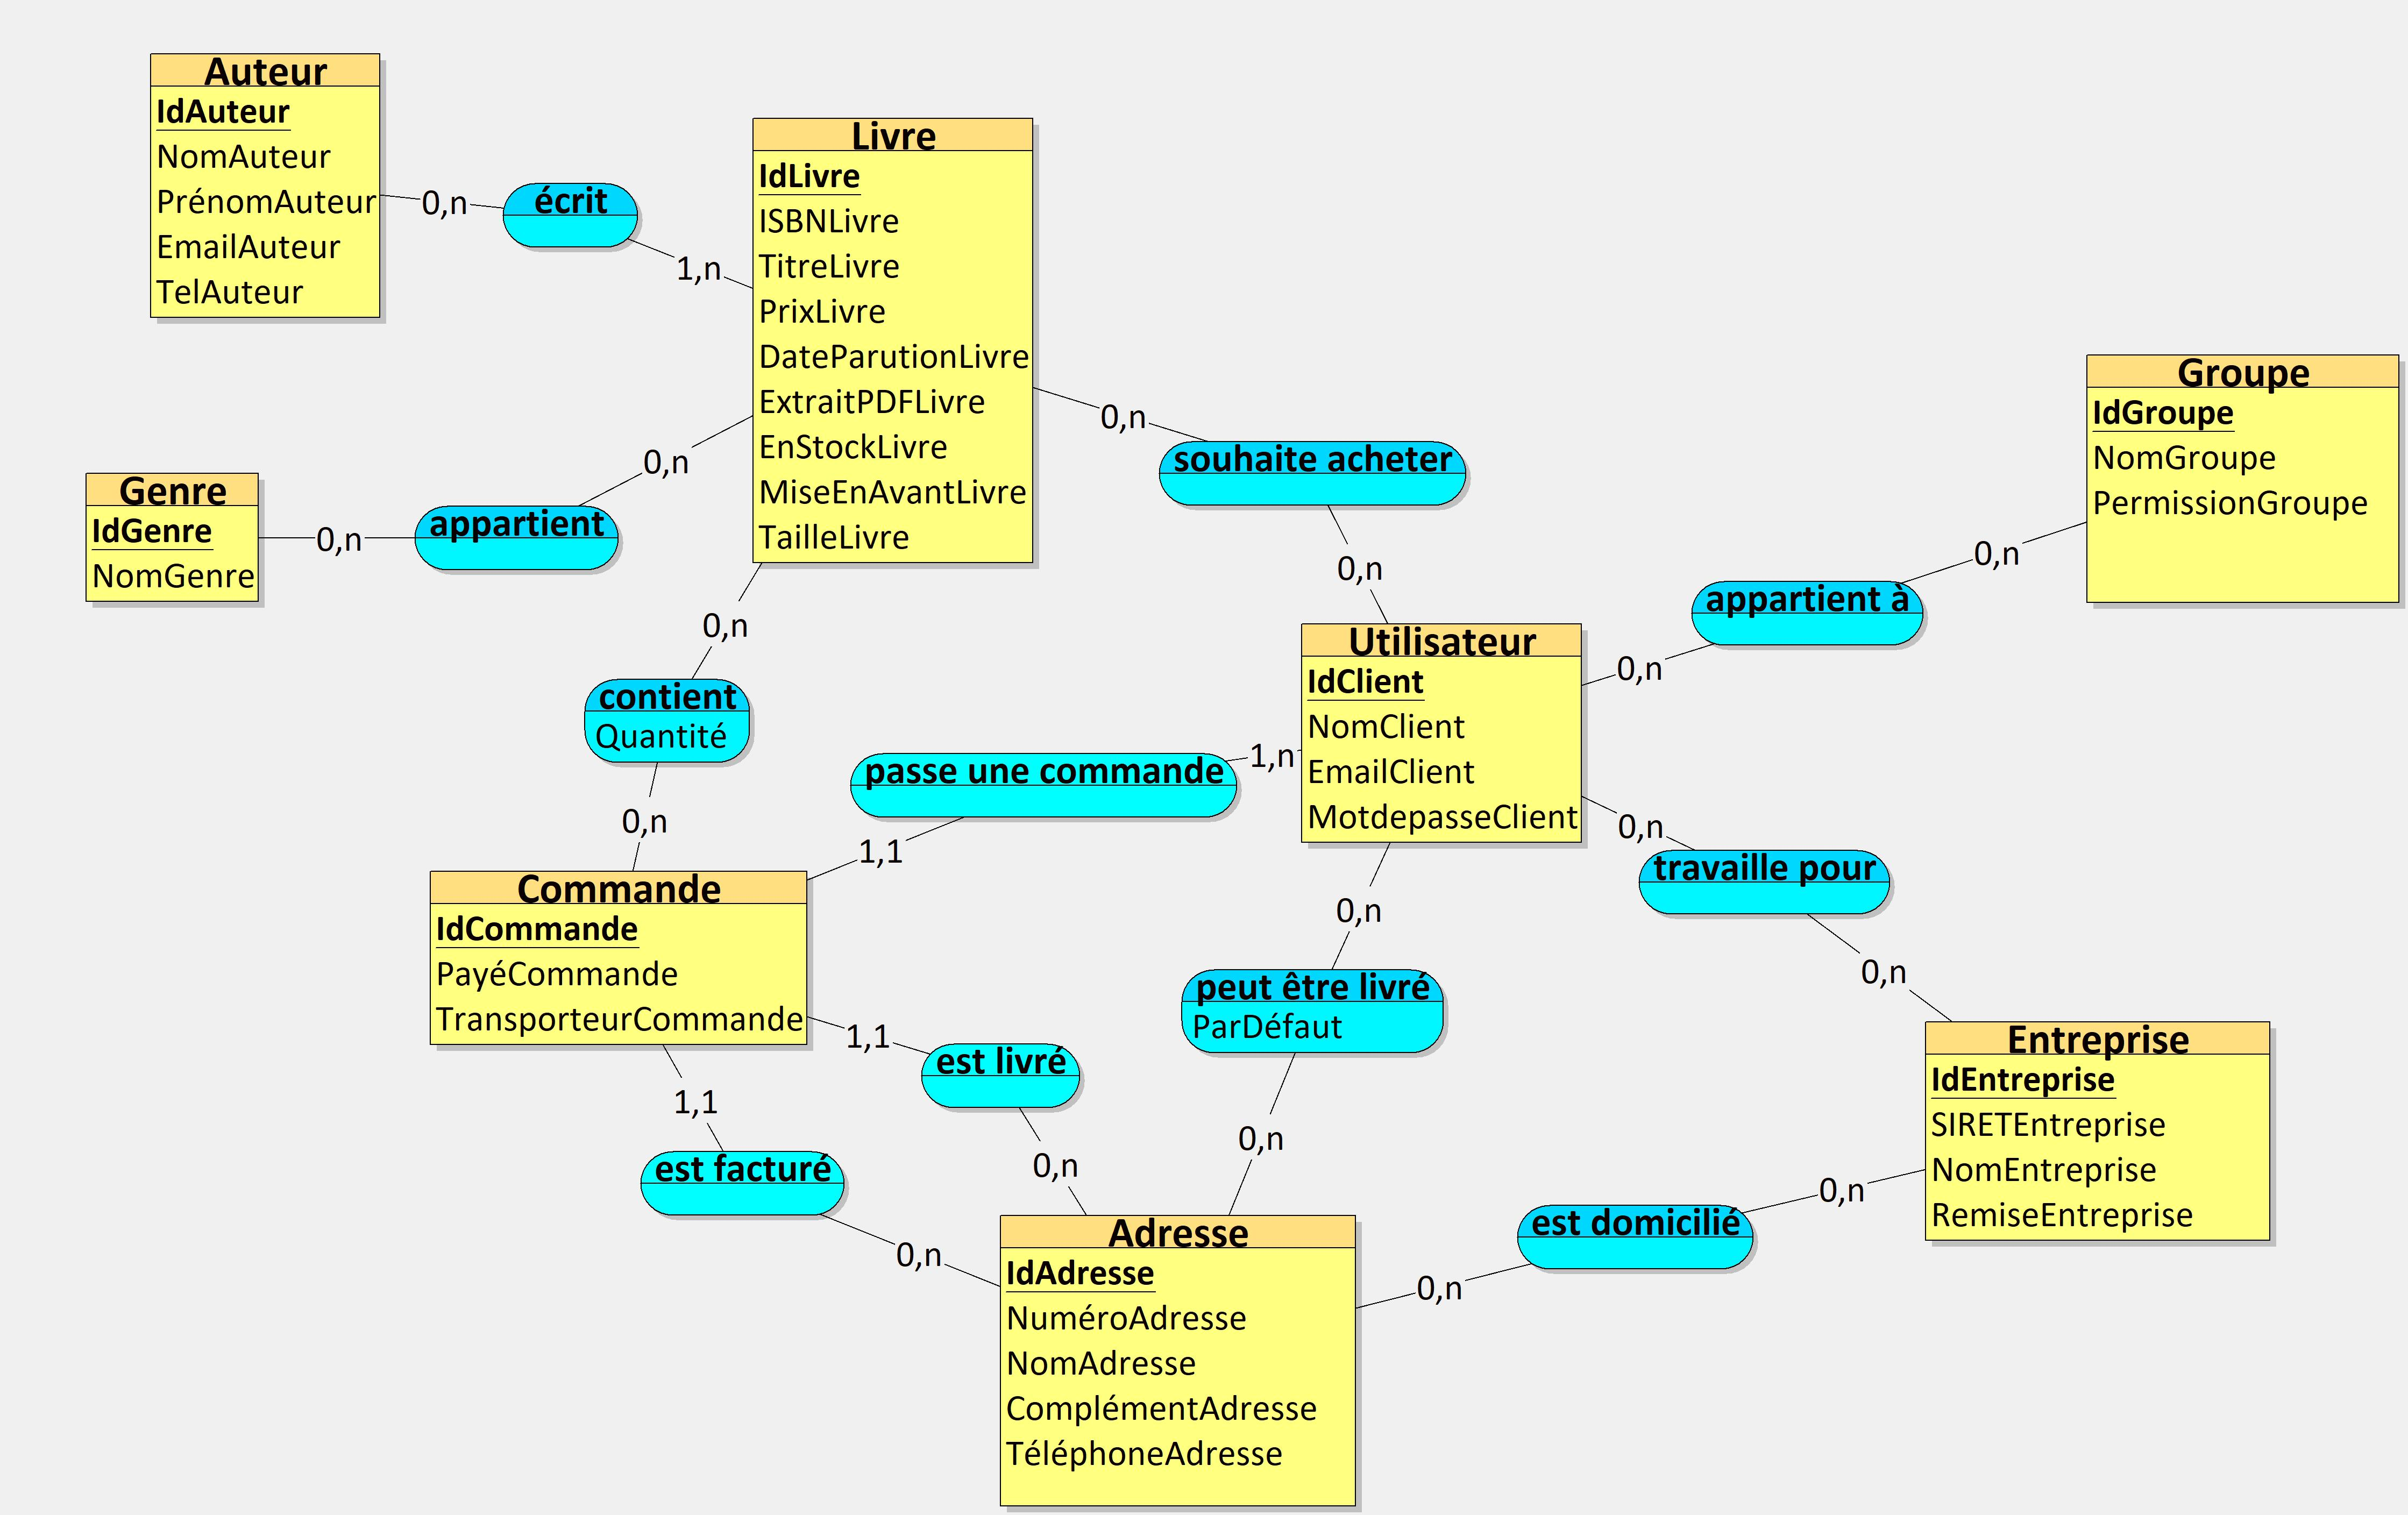
\includegraphics[width=0.8\linewidth]{images/mcd.jpg}
    \caption{Modèle conceptuelle de données}
\end{figure}
\end{document}   


